
\documentclass[aspectratio=169,11pt]{beamer}
\usetheme{Madrid}
\usecolortheme{seahorse}
\usefonttheme{professionalfonts}
\usepackage{amsmath,amssymb,bm,booktabs,array,graphicx,hyperref}
\usepackage{tikz}
\usetikzlibrary{positioning,arrows.meta,shapes.geometric,calc}
\usepackage{listings,xcolor,xeCJK,fontspec}
\graphicspath{{/mnt/data/week5_outputs_complete/}}
\setmainfont{DejaVu Sans}
\setsansfont{DejaVu Sans}
\setmonofont{DejaVu Sans Mono}
\setCJKmainfont{Noto Sans CJK SC}
\setCJKsansfont{Noto Sans CJK SC}
\setCJKmonofont{Noto Sans CJK SC}
\definecolor{myblue}{RGB}{36,88,135}
\definecolor{mygreen}{RGB}{40,120,80}
\definecolor{mygray}{RGB}{90,90,90}
\setbeamercolor{title}{fg=myblue}
\setbeamercolor{frametitle}{fg=myblue}
\setbeamercolor{structure}{fg=myblue}
\setbeamercolor{block title}{bg=myblue,fg=white}
\setbeamercolor{block body}{bg=blue!5,fg=black}
\setbeamertemplate{navigation symbols}{}
\setbeamertemplate{footline}[frame number]
\lstset{basicstyle=\ttfamily\scriptsize,keywordstyle=\color{myblue}\bfseries,stringstyle=\color{mygreen},commentstyle=\color{mygray},breaklines=true,frame=single,columns=fullflexible,keepspaces=true,showstringspaces=false}
\newcommand{\ind}{\mathbb{I}}
\title[Week 5]{Week 5: 传统 AI Baseline 与安全筛查指标}
\subtitle{Traditional ML baselines for three-phase microgrid N-1 screening}
\author{ECE Course: Physics-informed AI for Microgrid Security Prediction}
\date{}
\begin{document}
\begin{frame}\titlepage\end{frame}

\begin{frame}{本周学习目标}
\begin{enumerate}
  \item 将 Week 4 的三相 N-1 label 数据转化为监督学习数据集。
  \item 建立 pre-contingency feature set，并证明没有 target leakage。
  \item 训练 rule-based、logistic regression、random forest、gradient boosting 和 MLP baseline。
  \item 用 recall、FNR、AUPRC、PF calls saved 和 top-k recall 评价安全筛查器。
  \item 在 validation set 上选择高召回阈值，在 test set 上只评估一次。
  \item 比较 random split、scenario-group CV 和 contingency-group CV。
\end{enumerate}
\end{frame}

\begin{frame}{八周项目中的位置}
\centering
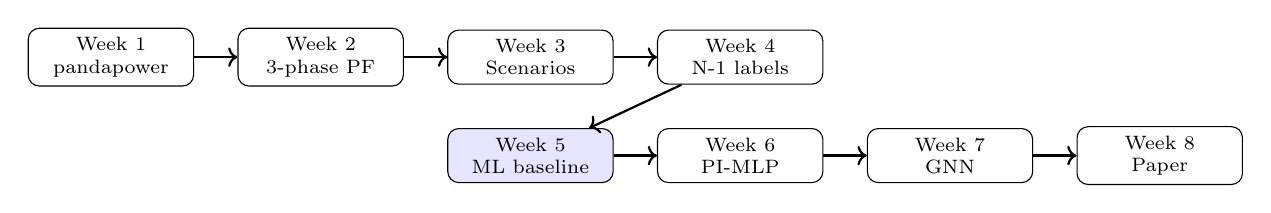
\begin{tikzpicture}[node distance=0.55cm, every node/.style={font=\scriptsize}]
\tikzstyle{box}=[draw, rounded corners, minimum width=2.1cm, minimum height=0.62cm, align=center]
\node[box] (w1) {Week 1\\pandapower};
\node[box, right=of w1] (w2) {Week 2\\3-phase PF};
\node[box, right=of w2] (w3) {Week 3\\Scenarios};
\node[box, right=of w3] (w4) {Week 4\\N-1 labels};
\node[box, below=of w3, fill=blue!10] (w5) {Week 5\\ML baseline};
\node[box, right=of w5] (w6) {Week 6\\PI-MLP};
\node[box, right=of w6] (w7) {Week 7\\GNN};
\node[box, right=of w7] (w8) {Week 8\\Paper};
\draw[->, thick] (w1)--(w2); \draw[->, thick] (w2)--(w3); \draw[->, thick] (w3)--(w4); \draw[->, thick] (w4)--(w5); \draw[->, thick] (w5)--(w6); \draw[->, thick] (w6)--(w7); \draw[->, thick] (w7)--(w8);
\end{tikzpicture}
\vspace{0.35cm}
\begin{block}{Week 5 的作用}把三相 N-1 数据变成可复现实验基线，为 Week 6/7 的物理约束模型提供比较对象。\end{block}
\end{frame}

\begin{frame}{从 Week 4 到 Week 5}
\begin{columns}
\begin{column}{0.48\textwidth}
\textbf{Week 4 输出}
\[(x_t,c_k) \mapsto (y_{t,k},s_{t,k})\]
\begin{itemize}\item operating scenario \item N-1 contingency \item safe / unsafe label \item severity score\end{itemize}
\end{column}
\begin{column}{0.48\textwidth}
\textbf{Week 5 输出}
\[\hat p_{t,k}=f_\theta(x_t,c_k)\]
\begin{itemize}\item violation probability \item high-recall threshold \item calls saved vs missed violations \item top-k ranking\end{itemize}
\end{column}
\end{columns}
\end{frame}

\begin{frame}{监督学习问题定义}
\begin{block}{Binary classification}\[\hat y_{t,k}(\tau)=\ind\{f_\theta(x_t,c_k)\ge \tau\}\]\end{block}
\begin{itemize}\item $\hat y=1$: 送入详细三相 N-1 潮流验证。\item $\hat y=0$: 暂时跳过或延后该 contingency。\item false negative: unsafe contingency 被错误跳过。\end{itemize}
\begin{alertblock}{安全重点}在安全筛查中，false negative 比 false positive 更危险。\end{alertblock}
\end{frame}

\begin{frame}{AI 筛查器在流程中的位置}
\centering
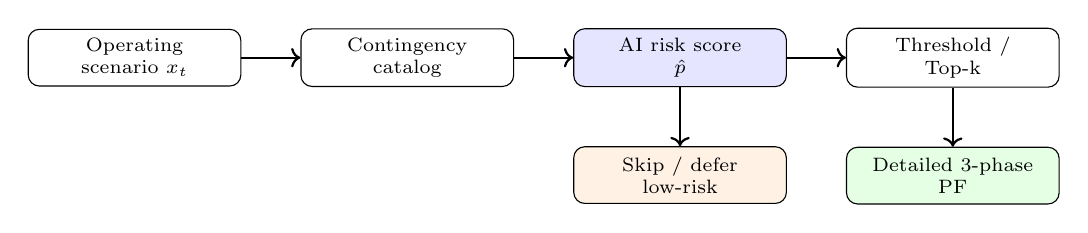
\begin{tikzpicture}[node distance=0.75cm, every node/.style={font=\scriptsize}]
\tikzstyle{box}=[draw, rounded corners, minimum width=2.7cm, minimum height=0.72cm, align=center]
\node[box] (scenario) {Operating\\scenario $x_t$};
\node[box, right=of scenario] (catalog) {Contingency\\catalog};
\node[box, right=of catalog, fill=blue!10] (ai) {AI risk score\\$\hat p$};
\node[box, right=of ai] (select) {Threshold /\\Top-k};
\node[box, below=of select, fill=green!10] (pf) {Detailed 3-phase\\PF};
\node[box, below=of ai, fill=orange!10] (skip) {Skip / defer\\low-risk};
\draw[->, thick] (scenario)--(catalog); \draw[->, thick] (catalog)--(ai); \draw[->, thick] (ai)--(select); \draw[->, thick] (select)--(pf); \draw[->, thick] (ai)--(skip);
\end{tikzpicture}
\vspace{0.3cm}
\begin{block}{核心定位}AI 不替代潮流求解器，而是作为 pre-screening module。\end{block}
\end{frame}

\begin{frame}{为什么不能只看 accuracy}
\begin{columns}
\begin{column}{0.48\textwidth}\textbf{普通分类任务}\begin{itemize}\item accuracy 常作为第一指标。\item 两类错误代价可能接近。\end{itemize}\end{column}
\begin{column}{0.48\textwidth}\textbf{安全筛查任务}\begin{itemize}\item false negative: 漏掉危险故障。\item false positive: 多运行一次潮流。\item 两者代价不对称。\end{itemize}\end{column}
\end{columns}
\begin{alertblock}{结论}Week 5 重点看 recall、FNR、missed violations 和 PF calls saved。\end{alertblock}
\end{frame}

\begin{frame}{混淆矩阵的工程解释}
\centering
\[\begin{array}{c|cc}& \hat y=0\;\text{skip} & \hat y=1\;\text{run PF} \\\hline y=0\;\text{safe} & TN & FP \\ y=1\;\text{unsafe} & FN & TP\end{array}\]
\begin{itemize}\item $TP$: 危险样本被送入详细潮流。\item $FP$: 安全样本被送入详细潮流，浪费计算。\item $TN$: 安全样本被跳过，节省计算。\item $FN$: 危险样本被跳过，最危险。\end{itemize}
\end{frame}

\begin{frame}{安全筛查指标}
\begin{columns}
\begin{column}{0.5\textwidth}\[\text{Recall}=\frac{TP}{TP+FN}\]\[\text{FNR}=\frac{FN}{TP+FN}=1-\text{Recall}\]\[\text{Precision}=\frac{TP}{TP+FP}\]\end{column}
\begin{column}{0.5\textwidth}\[\text{PF calls saved}=TN+FN\]\[\text{Saved ratio}=\frac{TN+FN}{N}\]\[\text{Workload}=\frac{TP+FP}{N}\]\end{column}
\end{columns}
\begin{alertblock}{解释}Saved ratio 必须和 missed violations 一起报告。\end{alertblock}
\end{frame}

\begin{frame}{High-recall threshold selection}
\[\tau^* = \arg\max_\tau \text{SavedRatio}_{val}(\tau),\quad \text{s.t. }\text{Recall}_{val}(\tau)\ge R_{target}\]
\begin{itemize}\item 默认 $R_{target}=0.95$。\item threshold 只能在 validation set 上选择。\item test set 只用于最后一次性能报告。\end{itemize}
\begin{alertblock}{实验纪律}如果在 test set 上调 threshold，就会造成评价泄漏。\end{alertblock}
\end{frame}

\begin{frame}{特征选择：允许 vs 禁止}
\begin{columns}
\begin{column}{0.48\textwidth}\textbf{允许}\begin{itemize}\item load scale, phase factors\item PV scale, BESS setpoint\item base-case min voltage\item base-case max loading\item base-case VUF\item contingency type / metadata\end{itemize}\end{column}
\begin{column}{0.48\textwidth}\textbf{禁止}\begin{itemize}\item post-contingency voltage\item post-contingency loading\item post-contingency VUF\item unserved load\item convergence flag\item violation flags\item label and severity\end{itemize}\end{column}
\end{columns}
\end{frame}

\begin{frame}[fragile]{No-leakage proof in Notebook}
\begin{lstlisting}[language=Python]
forbidden_tokens = [
    "converged", "min_vm", "max_vm", "max_vuf",
    "max_line_loading", "unserved", "violation",
    "severity", "pf_status",
]
leaky_features = [c for c in feature_cols
                  if is_forbidden_feature(c)]
assert not leaky_features
\end{lstlisting}
\begin{block}{证明目标}模型输入只能使用真实部署时刻能拿到的信息。\end{block}
\end{frame}

\begin{frame}{Dataset schema proof}
\begin{enumerate}\item row id 唯一。\item 每个 $(scenario, contingency)$ 只出现一次。\item target 是二元变量，且 safe / unsafe 都存在。\item severity 非负。\item violation flags 的 OR 与 final label 一致。\end{enumerate}
\begin{block}{本次数据集}样本数 $N=77$；unsafe = 47；safe = 30；pre-contingency features = 32。\end{block}
\end{frame}

\begin{frame}{Baseline hierarchy}
\begin{enumerate}\item \textbf{AllUnsafe}: 召回高但不省计算。\item \textbf{EngineeringRule}: 用 base-case stress 和 contingency type 构造规则分数。\item \textbf{LogisticRegression}: 线性、可解释。\item \textbf{RandomForest}: 非线性 tabular baseline。\item \textbf{GradientBoosting}: 强树模型 baseline。\item \textbf{MLP}: Week 6 neural model 起点。\end{enumerate}
\end{frame}

\begin{frame}{Feature preprocessing}
\begin{columns}\begin{column}{0.48\textwidth}\textbf{Numeric}\begin{itemize}\item median imputation\item standard scaling\end{itemize}\end{column}\begin{column}{0.48\textwidth}\textbf{Categorical}\begin{itemize}\item most-frequent imputation\item one-hot encoding\item handle unknown categories\end{itemize}\end{column}\end{columns}
\begin{block}{Pipeline 设计}所有模型使用相同 feature set 和 split，确保 baseline comparison 公平。\end{block}
\end{frame}

\begin{frame}[fragile]{Notebook training loop}
\begin{lstlisting}[language=Python]
for name, model in models.items():
    model.fit(X_train, y_train)
    val_score = model.predict_proba(X_val)[:, 1]
    tau = choose_high_recall_threshold(
        y_val, val_score, target_recall=0.95)
    test_score = model.predict_proba(X_test)[:, 1]
    report_metrics(y_test, test_score, tau)
\end{lstlisting}
\end{frame}

\begin{frame}{Random holdout split}
\centering
\begin{tabular}{lrrr}\toprule Split & Samples & Unsafe & Violation rate \\\midrule Train & 39 & 24 & 0.615 \\ Validation & 18 & 11 & 0.611 \\ Test & 20 & 12 & 0.600 \\\bottomrule\end{tabular}
\vspace{0.45cm}\begin{block}{局限}Random split 适合 debug，但还需要 group CV。\end{block}
\end{frame}

\begin{frame}{Holdout results}
\scriptsize\centering
\begin{tabular}{lrrrrrrr}\toprule Model & $\tau$ & Recall & Prec. & FNR & Saved & Missed & AUPRC \\\midrule
AllUnsafe & 0.000 & 1.000 & 0.600 & 0.000 & 0.000 & 0 & 0.600 \\
EngineeringRule & 0.650 & 1.000 & 0.857 & 0.000 & 0.300 & 0 & 0.910 \\
LogisticRegression & 0.735 & 0.833 & 1.000 & 0.167 & 0.500 & 2 & 1.000 \\
RandomForest & 0.677 & 0.833 & 0.909 & 0.167 & 0.450 & 2 & 0.956 \\
GradientBoosting & 0.301 & 1.000 & 1.000 & 0.000 & 0.400 & 0 & 1.000 \\
MLP & 0.000 & 1.000 & 0.600 & 0.000 & 0.000 & 0 & 0.533 \\
\bottomrule\end{tabular}
\vspace{0.2cm}\begin{block}{本次选择}Selected model: \textbf{GradientBoosting}, $\tau=0.301$。\end{block}
\end{frame}

\begin{frame}{Precision-recall curves}\centering
\includegraphics[width=0.82\textwidth]{week5_precision_recall_curves.png}\end{frame}
\begin{frame}{Recall vs threshold}\centering
\includegraphics[width=0.82\textwidth]{week5_recall_threshold_curves.png}\begin{block}{解释}阈值越高，模型越少判为 unsafe，计算量可能下降，但 recall 也可能下降。\end{block}\end{frame}
\begin{frame}{Saved PF calls vs missed violations}\centering
\includegraphics[width=0.82\textwidth]{week5_saved_calls_vs_missed_violations.png}\begin{alertblock}{解释}如果节省计算的代价是漏掉 unsafe contingency，则部署不可接受。\end{alertblock}\end{frame}

\begin{frame}{为什么需要 group-based CV}
\begin{columns}\begin{column}{0.48\textwidth}\textbf{Random split 问题}\begin{itemize}\item 相同 scenario family 可能进测试集。\item 相同 contingency family 可能进测试集。\item 泛化能力可能被高估。\end{itemize}\end{column}\begin{column}{0.48\textwidth}\textbf{Group CV 目标}\begin{itemize}\item scenario-group CV: unseen operating scenarios。\item contingency-group CV: unseen outages。\item 更接近论文泛化评估。\end{itemize}\end{column}\end{columns}
\end{frame}

\begin{frame}{Scenario-group CV}\[\mathcal{S}_{train}\cap\mathcal{S}_{test}=\emptyset\]\begin{itemize}\item 测模型是否能泛化到没有见过的 operating condition。\item Notebook 中每个 fold 都断言 train/test scenario 不重叠。\end{itemize}\end{frame}
\begin{frame}{Contingency-group CV}\[\mathcal{C}_{train}\cap\mathcal{C}_{test}=\emptyset\]\begin{itemize}\item 测模型是否能泛化到没有见过的 outage。\item 小数据集上通常更困难。\end{itemize}\end{frame}

\begin{frame}{Cross-validation summary}
\scriptsize\centering
\begin{tabular}{llrrrr}\toprule CV protocol & Model & Recall & FNR & Saved & AUPRC \\\midrule
contingency\_group & EngineeringRule & 1.000 & 0.000 & 0.310 & 0.971 \\
contingency\_group & LogisticRegression & 0.254 & 0.746 & 0.786 & 0.909 \\
contingency\_group & RandomForest & 0.400 & 0.600 & 0.690 & 0.861 \\
scenario\_group & EngineeringRule & 1.000 & 0.000 & 0.323 & 0.912 \\
scenario\_group & LogisticRegression & 0.928 & 0.072 & 0.439 & 0.990 \\
scenario\_group & RandomForest & 0.899 & 0.101 & 0.475 & 0.990 \\
\bottomrule\end{tabular}
\vspace{0.25cm}\begin{block}{解读}Random split 是 debug 结果；group CV 才能支持泛化声明。\end{block}
\end{frame}

\begin{frame}{Top-k screening}
\[\text{Top-}k(x_t)=\operatorname{argsort}_k f_\theta(x_t,c)\]
\[\text{ViolationRecall@}k=\frac{|\text{Top-}k\cap\mathcal{V}_t|}{|\mathcal{V}_t|}\]
\[\text{SevereHit@}k=\ind\{\arg\max_c s_{t,c}\in\text{Top-}k\}\]
\end{frame}

\begin{frame}{Top-k results}
\scriptsize\centering
\begin{tabular}{rrrrr}\toprule $k$ & Mean recall@k & Min recall@k & Severe hit@k & PF fraction \\\midrule
1 & 0.156 & 0.091 & 1.000 & 0.091 \\
2 & 0.312 & 0.182 & 1.000 & 0.182 \\
3 & 0.468 & 0.273 & 1.000 & 0.273 \\
5 & 0.779 & 0.455 & 1.000 & 0.455 \\
8 & 0.961 & 0.727 & 1.000 & 0.727 \\
10 & 0.987 & 0.909 & 1.000 & 0.909 \\
\bottomrule\end{tabular}
\vspace{0.25cm}\begin{block}{解释}Top-k 模式适合先验证最危险的若干 contingencies。\end{block}
\end{frame}
\begin{frame}{Top-k violation recall curve}\centering
\includegraphics[width=0.82\textwidth]{week5_topk_violation_recall.png}\end{frame}
\begin{frame}{Random forest feature importance}\centering
\includegraphics[width=0.78\textwidth]{week5_feature_importance.png}\begin{block}{提醒}Feature importance 不是因果解释，但能帮助检查模型是否依赖合理 stress indicators。\end{block}\end{frame}

\begin{frame}{Manual metric proof}
\[TP=\sum_i \ind\{y_i=1,\hat y_i=1\},\quad FP=\sum_i \ind\{y_i=0,\hat y_i=1\}\]
\[TN=\sum_i \ind\{y_i=0,\hat y_i=0\},\quad FN=\sum_i \ind\{y_i=1,\hat y_i=0\}\]
Notebook 会将手算结果与 sklearn confusion matrix 逐项对比。
\end{frame}

\begin{frame}{Validation suite}
Notebook validation summary: \textbf{12/12 checks passed}。
\begin{itemize}\item schema proof\item target has two classes\item no-feature-leakage proof\item split disjoint proof\item threshold chosen on validation proof\item manual confusion matrix proof\item group CV proof\item top-k and reproducibility proof\item output figures exist\end{itemize}
\end{frame}

\begin{frame}[fragile]{Notebook 输出文件}
\begin{lstlisting}
week5_baseline_dataset.csv
week5_holdout_results.csv
week5_cv_summary.csv
week5_validation_summary.csv
week5_screening_tradeoff.csv
week5_topk_violation_recall.csv
week5_precision_recall_curves.png
week5_recall_threshold_curves.png
week5_saved_calls_vs_missed_violations.png
week5_feature_importance.png
\end{lstlisting}
\end{frame}

\begin{frame}{课堂 lab 流程}
\begin{enumerate}\item 读取 Week 4 AI-ready dataset。\item 合并 Week 3 base-case features。\item 运行 schema proof 和 leakage guard。\item 训练 rule-based 和 ML baselines。\item 用 validation set 选择 threshold。\item 在 test set 上报告 safety metrics。\item 运行 scenario / contingency group CV。\item 导出结果表和图。\end{enumerate}
\end{frame}

\begin{frame}{学生练习}
\begin{enumerate}\item 加入 engineered feature，例如 distance to PCC 或 downstream load。\item 比较加入该 feature 前后的 recall、FNR 和 saved ratio。\item 将目标 recall 从 0.95 改成 0.90，观察节省计算量变化。\item 解释为什么 AllUnsafe baseline 重要。\end{enumerate}
\end{frame}

\begin{frame}{连接 Week 6: Physics-informed MLP}
\[\mathcal{L}_{data}=\mathrm{BCE}(y,\hat p)\]
\[\mathcal{L}=\mathcal{L}_{data}+\lambda_{lim}\mathcal{L}_{limit}+\lambda_{rank}\mathcal{L}_{rank}+\lambda_{cal}\mathcal{L}_{calibration}\]
\begin{itemize}\item Week 5 给出数据、指标和 baseline。\item Week 6 在此基础上加入物理约束和多任务损失。\end{itemize}
\end{frame}

\begin{frame}{本周 takeaway}
\centering\Large 安全预测模型的价值不是“分类准确”，而是在可控漏报风险下减少昂贵的三相 N-1 潮流计算。
\vspace{0.4cm}\[\text{high recall} + \text{low missed violations} + \text{useful PF-call reduction}\]
\end{frame}
\end{document}
